\documentclass{report}
\usepackage[utf8]{inputenc}
\usepackage[T1]{fontenc}
\usepackage[a4paper,margin=2.5cm,headheight=15pt]{geometry}
\usepackage{lmodern}
\usepackage{parskip,enumitem,float,graphicx,caption}
\usepackage{booktabs,array,tabularx,longtable,amsmath}
\usepackage{xcolor,listings,tikz}
\usetikzlibrary{arrows.meta,positioning,fit,backgrounds,calc}
\usepackage{xurl}
\usepackage[hidelinks]{hyperref}
\usepackage{fancyhdr}
\hypersetup{pdftitle={IF4031 M1 - Sistem Koordinasi Kebencanaan},pdfauthor={Kelompok nasgor}}
\pagestyle{fancy}
\fancyhf{}
\fancyhead[L]{\small IF4031 -- Kelompok nasgor}
\fancyhead[R]{\small\nouppercase{\leftmark}}
\fancyfoot[C]{\thepage}
\renewcommand{\chaptermark}[1]{\markboth{Bab \thechapter}{}}
\setlength{\emergencystretch}{3em}
\setlength{\tabcolsep}{5pt}
\renewcommand{\arraystretch}{1.2}
\setlist{nosep,topsep=5pt,leftmargin=*}
\setcounter{tocdepth}{1}
\definecolor{reportblue}{HTML}{224B68}
\definecolor{codebg}{HTML}{F4F5F6}
\lstset{basicstyle=\ttfamily\footnotesize,backgroundcolor=\color{codebg},breaklines=true,columns=fullflexible,keepspaces=true,showstringspaces=false,frame=single,rulecolor=\color{black!15},xleftmargin=4pt,xrightmargin=4pt,aboveskip=8pt,belowskip=8pt}
\DeclareRobustCommand{\code}[1]{\nolinkurl{#1}}
\newcolumntype{P}[1]{>{\raggedright\arraybackslash}p{#1}}
\renewcommand{\tabularxcolumn}[1]{>{\raggedright\arraybackslash}p{#1}}
\newcolumntype{Y}{>{\raggedright\arraybackslash}X}
\renewcommand{\contentsname}{Daftar Isi}
\renewcommand{\chaptername}{Bab}
\renewcommand{\figurename}{Gambar}
\renewcommand{\tablename}{Tabel}
\renewcommand{\bibname}{Daftar Pustaka}
\renewcommand{\appendixname}{Lampiran}
\graphicspath{{images/}}
% Screenshot asli dipertahankan; ukuran dibatasi agar caption tetap satu halaman.
\newcommand{\evidencefigure}[3]{%
\begin{figure}[htbp]\centering
\includegraphics[width=.97\linewidth,height=.66\textheight,keepaspectratio]{#1}
\caption{#2}\label{#3}
\end{figure}}


\hypersetup{
    colorlinks=true,
    linkcolor=black,
    filecolor=magenta,
    urlcolor=cyan,
    pdftitle={Tugas Besar IF4031 Arsitektur Aplikasi Terdistribusi},
}
\hypersetup{pageanchor=false}
\begin{document}

\begin{titlepage}
    \centering

    \Large \textsf{Tugas Besar IF4031 Arsitektur Aplikasi Terdistribusi} \\
    \vspace{1.5cm}

    \huge \textbf{systemname \\ Sistem Koordinasi Kebencanaan} \\
    \vspace{1.5cm}

    
\includegraphics[width=0.4\textwidth]{cover.jpeg} \\
    \vspace{1.5cm}

    \large \textit{Disusun oleh: nasgor} \\
    \vspace{0.5cm}

    \begin{tabular}{r l}
        Muhammad Aulia Azka & 13523137 \\
        Arlow Emmanuel Hergara & 13523161 \\
        Fachriza Ahmad Setiyono & 13523162
    \end{tabular}

    \vfill

    \large
    Program Studi Teknik Informatika \\
    Sekolah Teknik Elektro dan Informatika \\
    Institut Teknologi Bandung \\
    2026
\end{titlepage}

\pagenumbering{roman}
\begin{table}[H]
    \centering
    \small
    \begin{tabular}{@{} p{2.5cm} p{4.5cm} p{4.5cm} @{} }
        \toprule
        \textbf{NIM} & \textbf{Nama} & \textbf{Kontribusi} \\ \midrule
        \textbf{13523137} & Muhammad Aulia Azka & test \\ \midrule
        \textbf{13523161} & Arlow Emmanuel Hergara & bsea \\ \midrule
        \textbf{13523162} & Fachriza Ahmad Setiyono & Lorem ipsum dolor sit amet, consectetur adipiscing elit, sed do eiusmod tempor incididunt ut labore et dolore magna aliqua. Ut enim ad minim veniam, quis nostrud exercitation ullamco laboris nisi ut aliquip ex ea commodo consequat. Duis aute irure dolor in reprehenderit in voluptate velit esse cillum dolore eu fugiat nulla pariatur. Excepteur sint occaecat cupidatat non proident, sunt in culpa qui officia deserunt mollit anim id est laborum.
        \\ \bottomrule
    \end{tabular}
    \caption{Tabel Kontribusi}
\end{table}
\tableofcontents
\newpage

\hypersetup{pageanchor=true}
\pagenumbering{arabic}

\chapter{Gambaran Sistem}
\section{Tujuan dan Ruang Lingkup Milestone 1}
\NamaSistem{} mengintegrasikan kejadian gempa dan aktivitas gunung api dari mock BMKG dan PVMBG menjadi \code{HazardEvent} kanonik. BNPB mengambil data dengan polling, menyimpan hasil normalisasi, menyediakan API bagi klien, dan mendistribusikan publikasi yang sama kepada layanan live feed, webhook, serta notifikasi bahaya. Pengguna terdiri atas Media, Tim Lapangan, dan BNPB Pusat; hak akses ditentukan server berdasarkan identitas masing-masing.

Milestone ini berfokus pada interoperabilitas data (P1), isolasi kelambatan dan kegagalan sumber (P2), autentikasi dan otorisasi (P3), pemisahan layanan beserta penyimpanannya (P4), dan distribusi event melalui pub/sub (P5), sesuai spesifikasi tugas~\cite{spec}. Data bencana adalah simulasi untuk pengujian, bukan informasi operasional kebencanaan. Klien membaca data hazard; operasi tulis terbatas pada pengaturan langganan, sesi, dan kontrol mock untuk demo.

Laporan diperbarui pada 10 Oktober 2026 berdasarkan snapshot repository \code{4a1973b}, termasuk bukti manual P1--P5, dua keluaran k6, laporan suite otomatis, serta empat screenshot tambahan P3/P4. Bukti baru memperlihatkan penolakan kredensial silang, refresh sesi OIDC pada browser, dan build Notification dengan \code{--no-deps}. Bukti historis tetap dicantumkan dengan tanggal aslinya. Penjelasan implementasi ditelusuri ke kode dan Compose pada snapshot tersebut; pembaruan dokumen tidak menjalankan ulang pengujian. Cakupan bukti dijelaskan pada bab terkait; inventaris berkas tersedia di \code{docs/tex/evidence/manifest.json}.

\section{Arsitektur dan Batas Layanan}
Gambar~\ref{fig:architecture} menunjukkan seluruh container pada stack utama beserta arah komunikasinya. Kotak BMKG dan PVMBG di bagian atas adalah sistem sumber di luar BNPB; masing-masing hanya diwakili gateway mock. Kotak putus-putus di dalam BNPB mengelompokkan container yang diinstrumentasi dan dipantau, sedangkan Blackbox Exporter dan OTEL LGTM berada di luarnya sebagai komponen observabilitas. Tanda \emph{DB} menandakan penyimpanan milik container tersebut: SQLite privat pada mock, Webhook Provider, dan Danger Notification; PostgreSQL canonical store pada Aggregator; serta PostgreSQL Auth pada Zitadel. Kedua PostgreSQL berjalan sebagai container database terpisah dengan pemilik logis tunggal, bukan database bersama. Panah mengikuti arah pemanggil ke penerima, kecuali panah dari Message Broker yang mengikuti aliran publikasi.

\begin{figure}[H]
\centering
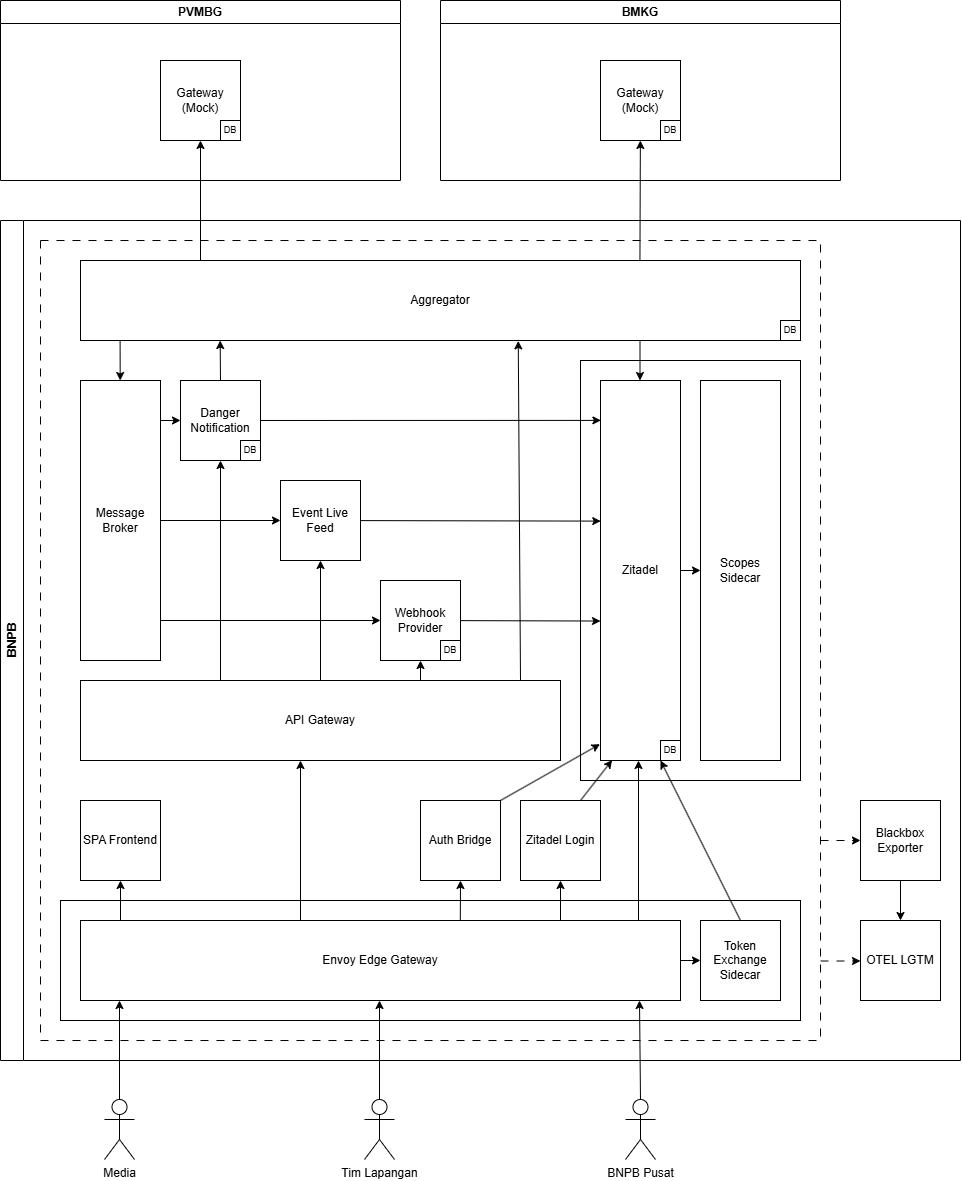
\includegraphics[width=.9\linewidth,height=.72\textheight,keepaspectratio]{architecture}
\caption{Arsitektur container \NamaSistem{}. Panah REST/gRPC mengikuti pemanggil ke penerima; panah dari Message Broker mengikuti aliran publikasi AMQP; panah putus-putus menunjukkan probe dan telemetri.}
\label{fig:architecture}
\end{figure}

\begin{enumerate}
\item Media, Tim Lapangan, dan BNPB Pusat mengakses satu origin melalui Envoy Edge Gateway. Envoy meneruskan \code{/} ke SPA Frontend (Nginx), \code{/auth/*} ke Auth Bridge, halaman login ke Zitadel Login, serta request OIDC ke Zitadel. Tidak ada jalur langsung dari pengguna ke container lain.
\item Untuk setiap request \code{/api/}, Envoy memanggil Token Exchange Sidecar (Rust) melalui \code{ext_authz}. Sidecar menukar access token opaque milik pengguna dengan JWT ke Zitadel (RFC 8693), lalu Envoy meneruskan request beserta JWT tersebut ke API Gateway.
\item API Gateway (Go) menerjemahkan REST/JSON dan SSE menjadi pemanggilan gRPC ke Aggregator, Danger Notification, Event Live Feed, dan Webhook Provider. Pembacaan hazard mengambil canonical store melalui Aggregator, bukan memanggil mock secara sinkron.
\item Aggregator melakukan polling REST/JSON ke kedua mock dengan kredensial berbeda. Tidak ada push langsung dari mock ke BNPB. Hasil normalisasi dan outbox ditulis dalam satu transaksi PostgreSQL; publisher mengirim envelope Protobuf dari outbox ke Message Broker (RabbitMQ).
\item Message Broker membagikan publikasi ke queue tiap consumer. Event Live Feed menyediakan replay dan stream, Webhook Provider mengirim HTTP callback ke endpoint eksternal, dan Danger Notification menyimpan notifikasi serta push outbox sebelum worker mengirim melalui Firebase Cloud Messaging (FCM). Danger Notification juga memanggil Aggregator untuk status kesegaran sumber. Endpoint webhook dan FCM berada di luar sistem sehingga tidak digambarkan.
\item Aggregator, Danger Notification, Event Live Feed, dan Webhook Provider memverifikasi JWT secara mandiri memakai metadata dan kunci publik Zitadel. Role dan scope pada JWT dipasok Zitadel melalui Scopes Sidecar (\code{zitadel-claims}, target Actions v2).
\item Seluruh container di dalam kotak putus-putus mengirim trace, metric, dan log melalui OpenTelemetry ke OTEL LGTM. Blackbox Exporter melakukan probe HTTP/gRPC/TCP ke container tersebut dan hasilnya di-scrape oleh OTEL LGTM.
\end{enumerate}

Kelompok komponen \emph{Auth} pada rancangan awal direalisasikan oleh Zitadel, Zitadel Login, Auth Bridge, Token Exchange Sidecar, dan Scopes Sidecar. Auth Bridge hanya menangani \code{/auth/*} (OIDC dan sesi SQLite terenkripsi); permintaan API bisnis melewati Envoy dan API Gateway. Container sekali jalan \code{auth-bootstrap}, yang menyiapkan proyek, akun, grant, dan client OIDC sebelum layanan lain berjalan, tidak digambarkan karena tidak aktif saat runtime. Observabilitas menggunakan container \code{otel-lgtm} serta \code{blackbox}, bukan container Prometheus dan Jaeger terpisah seperti sketsa awal.

\section{Teknologi dan Alasan Pemilihan}
\begin{longtable}{@{}P{3cm}P{3.6cm}P{8.2cm}@{}}
\toprule \textbf{Komponen} & \textbf{Teknologi} & \textbf{Alasan dan tanggung jawab}\\\midrule\endhead
BMKG dan PVMBG & Python 3.12, HTTP standard library, SQLite & Dependensi ringan; thread request memungkinkan health/admin tetap merespons saat request data menunggu. File database mempertahankan seed dan event setelah restart.\\
Frontend & React, TypeScript, Vite, Nginx & SPA dengan tampilan login, filter/daftar/detail hazard, status sumber, live feed, notifikasi, dan webhook; Nginx menyajikan hasil build statis.\\
Edge dan REST API & Envoy, Rust (Tonic); Go, chi, oapi-codegen & Envoy melakukan routing; sidecar Rust menukar token melalui \code{ext_authz}. Go menjaga bentuk JSON, status HTTP, validasi OpenAPI, dan framing SSE yang berbeda dari ProtoJSON.\\
Aggregator & Go, gRPC, PostgreSQL 17 & Goroutine untuk polling independen; transaksi dan indeks relational untuk data inti, JSONB untuk atribut dinamis.\\
Event Live Feed & Rust, Tokio, Tonic & Stream asinkron dan buffer replay berbatas; API Gateway mengubahnya menjadi SSE untuk browser.\\
Webhook Provider & Go, SQLite WAL & Menyimpan subscription, hasil delivery, dan deduplikasi; worker mengirim HTTP callback bertanda tangan.\\
Danger Notification & C\#, ASP.NET gRPC, EF Core SQLite, Firebase Admin & Menyimpan notifikasi dan push outbox privat, menyediakan proyeksi summary/full, serta mengirim push FCM melalui worker. Status kesegaran sumber dibaca melalui Aggregator.\\
Identitas & Zitadel, PostgreSQL, Node.js 24, Rust & Provider mengelola akun; bridge menjalankan OIDC dan sesi SQLite terenkripsi; Rust Actions memasok role/scope.\\
Distribusi event & RabbitMQ 4, AMQP, Protobuf & Fanout dan queue independen memisahkan produsen dari consumer serta menyediakan acknowledgement.\\
Observabilitas & OpenTelemetry, otel-lgtm, blackbox exporter & Pengiriman trace/metric/log dan probe HTTP/gRPC/TCP; dashboard serta alert diprovisikan melalui berkas repo.\\
Orkestrasi & Docker Compose & Batas proses, jaringan, volume, dan dependensi dinyatakan di satu stack utama; Compose khusus dipakai untuk pengembangan parsial.\\\bottomrule
\end{longtable}

\section{Asumsi dan Konfigurasi}
\begin{enumerate}
\item Instalasi M1 berjalan pada satu host Docker. Port publik default adalah BNPB 8080, BMKG 8081, PVMBG 8082, Grafana 3000, serta RabbitMQ Management 15672. Port mock dalam container adalah 8080.
\item Host \code{localhost} dan \code{auth.localhost} menunjuk mesin demo. HTTP diizinkan secara eksplisit untuk lingkungan lokal; ini bukan konfigurasi TLS produksi.
\item Setiap mock menyiapkan minimal 20 record pada database baru. Interval event default 10 detik; polling contoh 3 detik. Semua nilai latensi konfigurasi merupakan parameter simulasi, bukan hasil benchmark.
\item ID sumber dan timestamp menjadi dasar watermark polling inklusif. Tabel referensi gunung statis merupakan data milik BNPB. Penerimaan field tambahan tidak menjamin kompatibilitas perubahan tipe atau penggantian nama field wajib.
\item Aggregator adalah pemilik logis canonical store untuk operasi bisnis. Layanan lain memakai gRPC atau event; Notification membaca notifikasi dari SQLite miliknya. Collector juga mengakses PostgreSQL untuk metrik. Distribusi environment Compose belum membatasi kredensial database secara eksklusif pada Aggregator; batas isolasi ini dijelaskan pada P4.
\item Akun pengguna di-seed pada Zitadel, bukan SQLite mock ataupun frontend. Tiga akun manusia memiliki role terpisah; service user untuk tes end-to-end memiliki kredensial tersendiri.
\item Notifikasi push memerlukan proyek Firebase dan service-account JSON lokal; konfigurasi web publik diperlukan untuk push browser. Tanpa dependensi tersebut, demo push belum dapat dianggap terbukti.
\item Restart mempertahankan volume bernama. Menghapus volume menghilangkan data persisten. Replay feed berada di memori, dan RabbitMQ belum memiliki mount data persisten eksplisit pada Compose saat ini.
\end{enumerate}

\section{Ringkasan Menjalankan Sistem}
Prasyarat dasar adalah Docker Desktop/Engine yang aktif dan Python 3.12+ untuk helper setup. Siapkan konfigurasi lokal dari contoh; helper mempertahankan secret yang sudah tersedia. Helper mock hanya mengisi dua kredensial sumber, sehingga nilai \code{REPLACE_*} lainnya dalam \code{.env} harus diprovisikan sesuai pemiliknya. Isi kredensial broker dan token internal yang digunakan; sesuaikan DSN database dengan definisi Compose. Sediakan file Firebase pada \code{FIREBASE_CREDENTIALS_PATH}. Nilai privat tidak dicantumkan dalam laporan.

\begin{lstlisting}
python tools/setup_mock_env.py
python tools/setup_auth_env.py
docker compose --env-file .env --env-file .env.auth -f compose.yaml config --quiet
docker compose --env-file .env --env-file .env.auth -f compose.yaml up --build -d --wait
\end{lstlisting}

Perintah terakhir merupakan satu perintah orkestrasi setelah prasyarat konfigurasi dipenuhi. Buka \url{http://localhost:8080}, pilih masuk melalui Zitadel, lalu gunakan akun \code{media-demo}, \code{lapangan-demo}, atau \code{bnpb-demo}. Password berasal dari \code{.env.auth}. Dashboard Compose utama menggunakan \code{VITE_DATA_MODE=gateway}; fixture lokal hanya untuk mode pratinjau/stack Auth terpisah. Login UI milik Zitadel tidak mengubah frontend BNPB menjadi SSR.

Panduan operasional tersedia di \code{README.md}, \code{docs/mock-testing.md}, \code{docs/auth-testing.md}, \code{docs/e2e-testing.md}, dan \code{docs/load-testing.md}. Untuk layanan BNPB yang sudah berkembang, gunakan Compose dan README layanan terbaru bila uraian status pada README root masih tertinggal. Stack parsial \code{compose.mocks.yaml}, \code{compose.auth.yaml}, serta \code{compose.frontend.yaml} tetap berguna untuk pengembangan, tetapi bukan pengganti pengujian integrasi stack utama.

\section{Strategi Verifikasi}
Artefak pengujian tersimpan di \code{docs/tex/evidence/}, meliputi hasil tes mock, tes browser Auth, unit test Aggregator, ringkasan pengujian otomatis, serta JSON k6. Screenshot demonstrasi dikelompokkan pada direktori P1--P5 sesuai problem yang diuji. Path singkat seperti \code{P3/1-new.png} relatif terhadap direktori bukti tersebut; path berawalan \code{evidence/} relatif terhadap \code{docs/tex/}. Nama berkas dan hash setiap artefak tercantum pada \code{docs/tex/evidence/manifest.json}.

Bukti terdiri atas inspeksi implementasi, hasil tes otomatis tersimpan, tangkapan layar demo, dan pengukuran k6. Bab P1--P5 menyajikan hasil aktual beserta rujukan artefaknya. Hasil k6 mencatat beban 50 VU selama 60 detik dan isolasi latensi BMKG; screenshot RabbitMQ memperlihatkan fanout serta penumpukan dan pengurasan backlog consumer. Status PASS pada suite otomatis dilaporkan sebagai hasil suite dengan cakupan assertion yang dijalankan, bukan pengganti setiap observasi manual. Bukti browser Auth historis dibedakan dari pengujian token API terbaru. Gambar yang menampilkan nilai secret konfigurasi tidak direproduksi dalam PDF.

\chapter[P1: Interoperabilitas Data]{P1: Arsitektur dan Interoperabilitas Data}
\section{Rancangan Solusi}
\subsection{Kontrak Sumber dan Akuisisi Data}
BMKG menyediakan \code{GET /seismic-events} dan \code{GET /tsunami-warnings}; PVMBG menyediakan \code{GET /volcanic-reports}. Ketiganya menerima \code{since} ISO 8601 yang inklusif dan mengembalikan koleksi \code{items}. Aggregator tidak meminta sumber mengikuti satu skema baru. Adapter per sumber memahami format asli, mengambil data dengan HTTP, lalu mengubahnya menjadi \code{HazardEvent}. Kontrak sumber didokumentasikan dalam \code{contracts/openapi/bmkg.yaml} dan \code{contracts/openapi/pvmbg.yaml}; kontrak keluaran publik ada pada \code{contracts/openapi/gateway.yaml}.

Kedua mock menggunakan SQLite file dengan kolom ID, waktu terindeks, dan payload JSON. Inisialisasi membuat tabel serta minimal 20 record ketika penyimpanan belum berisi data; seed tidak ditambahkan ulang pada setiap restart. Generator menambah satu event per interval, default 10 detik. BMKG memakai pola variasi berdasarkan indeks dan UUID untuk ID baru; tidak seluruh nilai gempa dibangkitkan acak. PVMBG memilih variasi laporan dengan bilangan acak, termasuk \code{confidence_level} ketika skema v2 aktif. Delay BMKG tetap, default 100 ms; delay PVMBG diambil acak antara 500--3000 ms. Sumber implementasi adalah \code{app.py}, \code{config.py}, dan \code{storage.py} pada direktori masing-masing mock.

\subsection{Model Kanonik dan Pemetaan}
\code{HazardEvent} memisahkan atribut lintas sumber dari rincian mentah. Tujuh field ringkasan adalah \code{hazard_id}, \code{source}, \code{hazard_type}, \code{severity}, \code{area_name}, \code{occurred_at}, dan \code{ingested_at}. Tampilan penuh menambahkan \code{source_ref_id}, \code{latitude}, \code{longitude}, serta \code{attributes}. BNPB memberikan ID kanonik dan waktu ingest saat menyimpan record. Unique key pasangan sumber dan ID asli menjaga identitas kanonik pada pengambilan berulang.

\begin{table}[H]\small
\begin{tabularx}{\textwidth}{@{}P{2.5cm}YY@{}}
\toprule \textbf{Field kanonik} & \textbf{BMKG} & \textbf{PVMBG}\\\midrule
\code{source} & BMKG & PVMBG\\
\code{source_ref_id} & \code{event_id} & \code{report_id}\\
\code{hazard_type} & SEISMIC & VOLCANIC\\
\code{area_name} & \code{region_name} & Nama gunung dari referensi BNPB berdasarkan \code{volcano_id}.\\
Koordinat & \code{epicenter_lat}, \code{epicenter_lon} & Koordinat referensi gunung statis.\\
\code{occurred_at} & \code{occurred_at} & \code{reported_at}\\
\code{severity} & Tingkat warning terkait; jika tidak ada, berdasarkan magnitudo. & Normal/Waspada/Siaga/Awas menjadi enum huruf kapital.\\
\code{attributes} & Magnitudo, kedalaman, potensi tsunami, daftar warning, dan tambahan sumber. & Jumlah erupsi, tinggi kolom abu, ID gunung, confidence bila ada, dan tambahan sumber.\\\bottomrule
\end{tabularx}
\caption{Pemetaan ke model kanonik pada adapter Aggregator.}
\end{table}

\code{BMKGPoller} mengambil gempa serta warning melalui endpoint terpisah, lalu membentuk indeks warning menurut \code{related_event_id}. Warning dihubungkan ke \code{event_id} sebelum normalisasi. Jika terdapat lebih dari satu warning, tingkat terberat dipilih dengan urutan AWAS, SIAGA, WASPADA. Tanpa warning, magnitudo $m<5{,}0$ menghasilkan NORMAL, $5{,}0\leq m<6{,}5$ WASPADA, dan $m\geq6{,}5$ SIAGA. Rincian warning disimpan sebagai array \code{attributes.tsunami_warnings}, sehingga informasi korelasi tetap tersedia pada proyeksi penuh.

Pemetaan PVMBG memakai \code{LookupVolcano} di \code{services/aggregator/internal/domain/volcano.go}. Implementasi menormalkan ID ke huruf kecil dan menerima awalan \code{v-}. Referensi memuat nama serta koordinat; dengan demikian mock tidak harus menambahkan field lokasi ke kontrak aslinya. Implementasi pemetaan kedua sumber berada di \code{services/aggregator/internal/ingest/mapper.go}.

\subsection{Perubahan Skema saat Runtime}
Operator mengirim \code{POST /admin/schema-version} dengan \verb|{"version":2}| pada PVMBG. Pengaturan ini memengaruhi laporan yang dibuat selanjutnya, tanpa restart. Laporan lama tetap tidak memiliki \code{confidence_level}; laporan baru menyimpan nilai tersebut dalam JSON SQLite. Mengembalikan versi menjadi 1 tidak menghapus field yang telah tersimpan pada laporan v2.

Decoder Aggregator memiliki field \code{ConfidenceLevel} opsional sekaligus map \code{RawFields}. JSON dibaca menjadi struktur bertipe untuk field inti dan map untuk field tambahan. Field yang sudah dikenal dikeluarkan dari map, sedangkan field tidak dikenal diteruskan ke \code{attributes}. Kebijakan ini berlaku pada gempa, warning tsunami, dan laporan vulkanik. Nilai confidence yang tidak ada dibedakan dari nilai numerik 0. PostgreSQL menyimpan atribut dalam JSONB tanpa menambah kolom; kontrak internal membawa atribut melalui struktur dinamis Protobuf. Pemanfaatan JSONB ini sesuai kemampuan penyimpanan dan pemrosesan JSON pada PostgreSQL~\cite{postgres}.

\section{Justifikasi dan Alternatif}
Model kanonik menghindarkan klien dari keharusan memahami dua format, dua kredensial sumber, serta aturan korelasi tsunami. Adapter terpisah membuat perubahan pada satu sumber tidak harus merombak API publik. Alternatif meneruskan payload mentah apa adanya lebih singkat untuk dibuat, tetapi setiap klien harus menduplikasi pemetaan dan pemisahan akses Media.

Struktur inti bertipe dengan map tambahan dipilih sebagai kompromi. Deserialisasi sangat ketat yang menolak semua field baru dapat menghentikan ingest ketika confidence mulai muncul. Sebaliknya, map bebas untuk seluruh record memindahkan kesalahan tipe dan field wajib ke tahap yang lebih jauh. Implementasi saat ini mempertahankan tipe inti dan menggunakan map untuk perubahan aditif. Field tambahan dapat ditelusuri kembali dalam proyeksi penuh, tanpa memperluas tujuh field ringkasan Media.

Polling mengikuti spesifikasi dan memudahkan pengujian sumber yang tidak menyediakan push. Watermark mengurangi pengambilan data berulang, sementara upsert melindungi identitas record. Konsekuensinya, data yang terlihat klien tertinggal setidaknya selama waktu tunggu polling dan pemrosesan; sistem ini bukan integrasi real-time dengan jaminan keterlambatan nol.

\section{Batasan Solusi}
\begin{itemize}
\item Dukungan perubahan aditif tidak otomatis menangani rename, penghapusan field wajib, atau perubahan tipe, misalnya \code{magnitude} menjadi objek. Perubahan semantik tersebut memerlukan pembaruan adapter dan kontrak.
\item Field yang tidak dikenal diteruskan, tetapi tidak otomatis dipahami secara bisnis. Penambahan nama yang bertabrakan dengan key atribut hasil normalisasi perlu kebijakan validasi yang lebih tegas.
\item ID gunung yang tidak ditemukan menggunakan ID asli sebagai nama area dan koordinat 0,0. Nilai ini merupakan fallback implementasi, bukan koordinat valid yang sudah diverifikasi.
\item Fetch warning BMKG dilakukan setelah fetch gempa. Error warning saat ini diabaikan, sehingga kejadian dapat dipetakan berdasarkan magnitudo tanpa pengayaan tsunami. Pembaruan warning untuk gempa yang sudah melewati watermark juga belum mempunyai alur pembaruan mandiri.
\item JSONB tidak menghilangkan kebutuhan validasi domain. Data tidak lengkap dan enum tidak dikenal belum memiliki karantina ingest yang menyeluruh.
\end{itemize}

\section{Proof-of-Concept dan Keterlacakan}
Pada 9 Oktober 2026 dijalankan tes paket Aggregator dengan \code{go test -json ./internal/ingest ./internal/domain ./internal/auth}. Tujuh tes tingkat utama paket ingest lulus, mencakup fetch HTTP kedua sumber, penolakan kredensial, pemetaan magnitudo, korelasi warning, evolusi skema, dan proyeksi data. Paket domain tidak memiliki test case dan tidak dihitung sebagai tes lulus. Rekaman ada dalam bukti E3 pada Lampiran~\ref{app:bukti}.

\begin{table}[H]\small
\begin{tabularx}{\textwidth}{@{}P{3.5cm}YY@{}}
\toprule \textbf{Kriteria} & \textbf{Bukti tersedia} & \textbf{Batas kesimpulan}\\\midrule
Pemetaan dua sumber & E3: tes mapping gempa/warning dan vulkanik lulus; \code{mapper_test.go}. & Membuktikan fungsi dengan input tes, belum seluruh alur Docker.\\
Skema v1/v2 dan field tambahan & E3: \code{TestMapPVMBGToHazard_SchemaEvolution}; E1: satu laporan v2 baru ditemukan saat kontrol runtime diubah. & E1 menguji mock; tes unit menguji mapper. Demo kontinu melalui gateway belum direkam.\\
Proyeksi kanonik & E3: \code{TestProjection_MediaVsFull} lulus. & Perlu E2E untuk mengikat proyeksi dengan role dan respons REST sesungguhnya.\\\bottomrule
\end{tabularx}
\caption{Bukti P1 yang tersedia dan batas cakupannya.}
\end{table}

Untuk melengkapi demo runtime, jalankan stack utama pada skema v1, rekam satu respons hazard vulkanik penuh beserta ID dan waktu ingest, ubah skema menjadi v2, lalu tunggu generator dan polling. Verifikasi hazard baru memiliki \code{attributes.confidence_level}, record lama tetap dapat dibaca, dan ID/start time container mock serta Aggregator tidak berubah. Request admin harus membawa bearer PVMBG dari konfigurasi lokal. Kembalikan skema ke v1 setelah demo. Simpan respons yang sudah disanitasi, correlation ID, serta log terkait; skenario ini belum diberi status lulus pada laporan.

\chapter{P2: Konkurensi dan Ketersediaan}
\label{chap:p2}

\section{Rancangan Solusi}

Sistem memisahkan pengambilan data sumber dari pelayanan permintaan pengguna.
Aggregator menjalankan poller BMKG dan PVMBG sebagai dua goroutine independen,
sementara layanan gRPC membaca data kanonis di PostgreSQL. Publisher outbox
berjalan pada goroutine lain. Pemisahan ini terlihat pada
\code{services/aggregator/cmd/main.go}. Dengan demikian, keterlambatan PVMBG
memengaruhi waktu pembaruan data PVMBG, bukan menambahkan waktu tunggu upstream
ke setiap pembacaan BMKG. Permintaan pengguna tetap bergantung pada kapasitas
gateway, autentikasi, Aggregator, dan database yang dipakai bersama.

Setiap poller melakukan pengambilan awal, kemudian mengulangi polling menurut
interval masing-masing. HTTP client memiliki timeout per sumber dan menerima
context untuk pembatalan saat layanan berhenti. Dalam satu poller, satu putaran
diselesaikan sebelum putaran berikutnya diproses; implementasi tidak membuat
goroutine baru tanpa batas pada setiap tick. BMKG mengambil seismic event lalu
peringatan tsunami secara berurutan, sedangkan PVMBG mengambil laporan vulkanik.
Implementasi berada pada \code{services/aggregator/internal/ingest/bmkg.go} dan
\code{services/aggregator/internal/ingest/pvmbg.go}.

\begin{table}[htbp]
    \centering
    \small
    \caption{Parameter konkurensi dan kesegaran data}
    \begin{tabularx}{\textwidth}{@{}P{0.30\textwidth}P{0.18\textwidth}X@{}}
        \toprule
        \textbf{Parameter} & \textbf{Nilai acuan} & \textbf{Makna} \\
        \midrule
        Interval polling kedua sumber & 3.000 ms & Contoh konfigurasi di \code{.env.example}. \\
        Timeout BMKG / PVMBG & 1.000 / 3.500 ms & Batas setiap request HTTP upstream, bukan target latensi API. \\
        Ambang stale & 10.000 ms & Acuan usia keberhasilan pengambilan sumber. \\
        Timeout unary gateway & 2.000 ms & Default deadline panggilan backend. \\
        Permintaan unary aktif & 100 & Default kapasitas semaphore gateway; stream dikecualikan. \\
        Koneksi PostgreSQL & 5--25 & Minimum dan maksimum pool Aggregator. \\
        \bottomrule
    \end{tabularx}
\end{table}

Setiap sumber mempunyai watermark, waktu keberhasilan terakhir, waktu percobaan
terakhir, dan pesan kegagalan. Setelah fetch berhasil, data dinormalisasi dan
disimpan sebelum watermark dimajukan. Pada kegagalan, data sebelumnya tidak
dihapus dan watermark keberhasilan dipertahankan. Pada pembacaan API,
\code{services/aggregator/internal/domain/status.go} menghitung status berikut:
\begin{itemize}
    \item \textbf{FRESH}: keberhasilan terakhir masih dalam ambang waktu dan
    tidak ada error sumber yang tercatat.
    \item \textbf{STALE}: sumber gagal atau terlalu lama tidak berhasil,
    tetapi data kanonis sumber tersebut masih tersedia.
    \item \textbf{UNAVAILABLE}: tidak tersedia data tersimpan untuk digunakan
    ketika sumber belum berhasil atau tidak dapat diperbarui.
\end{itemize}

Respons hazard tetap membawa item yang tersedia beserta metadata
\code{freshness}. Nilai \code{partial=true} diberikan apabila sumber yang
relevan dengan permintaan tidak fresh. Filter sumber membatasi pemeriksaan
kesegaran pada sumber tersebut. Mekanisme ini membedakan kondisi tidak ada
peristiwa dari sumber yang belum dapat memberikan data, sekaligus memungkinkan
klien menampilkan usia data. Pembentukan respons ada pada
\code{services/aggregator/internal/grpc/server.go}; penyimpanan watermark ada
pada \code{services/aggregator/internal/store/hazard_store.go}.

Gateway juga membatasi permintaan unary aktif dengan channel berkapasitas
tetap. Ketika penuh, permintaan ditolak dengan respons overload sesuai kontrak,
umumnya HTTP 429, dan \code{Retry-After}. Deadline unary membatasi waktu tunggu
backend. Pembatas ini bukan pembatas laju per pengguna dan tidak menghitung
stream SSE yang berumur panjang. Kode terkait adalah
\code{services/api-gateway/internal/server/server.go},
\code{services/api-gateway/internal/config/config.go}, dan
\code{services/api-gateway/internal/problem/problem.go}.

\section{Justifikasi dan Alternatif}

Polling independen dipilih karena data kebencanaan dikumpulkan secara berkala
dan dapat dilayani dari penyimpanan kanonis. Pengguna memperoleh respons dari
satu bentuk data meskipun kedua sumber memiliki latensi serta skema berbeda.
Biaya keputusan ini adalah jeda antara perubahan upstream dan kemunculannya
pada API. Karena itu, freshness merupakan bagian dari kontrak respons, bukan
sekadar informasi log.

Alternatif pertama ialah melakukan dua panggilan upstream secara serial pada
setiap request. Pendekatan tersebut sederhana, tetapi latensi sumber terakumulasi
dan gangguan satu sumber langsung memengaruhi request pengguna. Alternatif kedua
ialah fan-out paralel per request dengan deadline terpisah. Pendekatan kedua
mengurangi penjumlahan waktu tunggu, tetapi tetap menambah beban upstream
sebanding dengan jumlah pengguna dan memerlukan fallback tersendiri.

Penyimpanan kanonis dengan polling mengurangi keterikatan tersebut, dengan
konsekuensi kapasitas database menjadi sumber daya bersama. Pool koneksi dan
batas unary gateway menahan pertumbuhan pekerjaan aktif. Penggunaan circuit
breaker atau penjadwal polling terdistribusi dapat menjadi pengembangan
berikutnya, tetapi keduanya belum menjadi mekanisme yang digunakan pada
implementasi ini.

\section{Batasan Solusi}

Isolasi pada tingkat goroutine tidak menjamin isolasi CPU, memori, database,
atau autentikasi. Permintaan BMKG dan PVMBG tetap melewati komponen bersama.
Kegagalan PostgreSQL tidak dapat ditutupi oleh fallback memori karena jalur
baca kanonis masih membutuhkan database. Compose juga belum memberikan bukti
failover beberapa replika Aggregator atau database.

Status kesegaran BMKG terutama mengikuti keberhasilan seismic event. Error
pengambilan peringatan tsunami saat ini diabaikan oleh poller, sehingga
kegagalan pengayaan tsunami belum selalu muncul sebagai status stale.
Selain itu, pembaruan watermark dilakukan sesudah transaksi data selesai,
bukan di dalam transaksi yang sama. Restart pada sela kedua operasi dapat
menyebabkan data diambil kembali; kestabilan identitas hazard membantu menjaga
baris kanonis, tetapi tidak membuktikan tidak ada publication berulang.

Nilai timeout, kapasitas pool, serta semaphore merupakan konfigurasi atau
mekanisme yang ditemukan pada kode. Nilai tersebut tidak membuktikan target
p95, throughput, maupun tingkat availability tertentu tanpa pengukuran.
Tidak ada hasil uji beban gateway terbaru yang dilampirkan untuk snapshot
laporan 9 Oktober 2026.

\section{Proof-of-Concept dan Keterlacakan}

Bukti historis container pada 30 September 2026 disimpan dalam
\code{docs/tex/evidence/mock-container-2026-09-30.json}. Catatan tersebut memuat
10 pemeriksaan berhasil pada lingkup mock. Pengukuran langsung BMKG ketika
empat request PVMBG berjalan paralel tercatat 113,86 ms; pemeriksaan health dan
admin PVMBG tercatat masing-masing 22,29 ms dan 17,80 ms. Angka ini menunjukkan
perilaku pada skenario mock yang dicatat, bukan p95 gateway atau hasil
50 pengguna selama 60 detik.

\begin{table}[htbp]
    \centering
    \small
    \caption{Status pembuktian P2 pada snapshot laporan}
    \begin{tabularx}{\textwidth}{@{}P{0.25\textwidth}X P{0.20\textwidth}@{}}
        \toprule
        \textbf{Skenario} & \textbf{Target atau cakupan} & \textbf{Hasil} \\
        \midrule
        Konkurensi mock & Request BMKG bersamaan dengan empat request PVMBG & Bukti historis tersedia. \\
        Beban API lengkap & 50 VU, 60 detik; error tidak terkendali di bawah 1\%. Skrip juga menetapkan p95 di bawah 2 detik & Belum diukur. \\
        Isolasi melalui gateway & PVMBG ditunda 3 detik; p95 grup BMKG di bawah 300 ms & Belum diukur. \\
        Degradasi sumber & Data lama tetap terbaca dengan freshness yang sesuai & Mekanisme tersedia; hasil terbaru belum dilampirkan. \\
        \bottomrule
    \end{tabularx}
\end{table}

Repositori menyediakan skenario yang dapat diulang pada
\code{tests/load/aggregator.js} dan
\code{tests/load/aggregator-isolation.js}, dengan petunjuk pada
\code{docs/load-testing.md}. Prosedur pembuktian yang direncanakan adalah:
\begin{enumerate}
    \item Jalankan stack yang telah diprovisikan, pastikan akun layanan tersedia
    pada \code{.cache/auth/}, dan buat direktori \code{.cache/load/}.
    Jalankan \code{k6 run tests/load/aggregator.js} dari root repositori.
    Defaultnya adalah pemanasan 10 detik, lalu 50 VU selama 60 detik.
    Campuran request adalah 60\% daftar, 30\% detail, dan 10\% status sumber.
    Hanya fase beban dihitung; kegagalan pengambilan token dicatat terpisah.
    \item Untuk isolasi, tetapkan
    \code{PVMBG_RESPONSE_DELAY_MIN_MS} dan
    \code{PVMBG_RESPONSE_DELAY_MAX_MS} menjadi 3000, lalu buat ulang
    \code{pvmbg-mock} sebagaimana panduan. Jalankan
    \code{k6 run tests/load/aggregator-isolation.js}. Setup memeriksa tiga
    request langsung ke mock dan membatalkan pengujian bila median delay
    kurang dari 2900 ms.
    \item Bandingkan fase baseline 30 detik dengan fase kontensi 60 detik,
    setelah pemanasan 5 detik. Kedua fase menggunakan 10 VU BMKG yang diukur
    dan 10 VU kelompok kedua; kelompok kedua beralih dari BMKG ke PVMBG.
    Simpan p50/p95/p99, error, throughput, ringkasan JSON, dan jendela waktu
    untuk pencocokan trace. Pulihkan konfigurasi delay setelah selesai.
\end{enumerate}

Latensi yang diukur skrip tersebut mencakup Envoy, token exchange, gateway,
RPC, dan pembacaan database. Hasilnya harus dilaporkan sebagai latensi jalur API
lengkap. Keberadaan skrip, threshold, dan instrumen observabilitas merupakan
keterlacakan rancangan pengujian; belum merupakan hasil eksekusi pengujian.

Untuk menilai batas error spesifikasi, HTTP 429 yang merupakan backpressure
terkendali dilaporkan terpisah dari error tidak terkendali. Pada fase beban,
catat jumlah request API $N$, jumlah 429 $N_{429}$, dan kegagalan lain
$N_{\mathrm{err}}$; laporkan $100N_{\mathrm{err}}/N$ serta
$100N_{429}/N$. Denominator dan definisi kegagalan harus dicantumkan agar
angka dapat diperiksa. Threshold error bawaan skrip masih menghitung 429,
sehingga lebih ketat daripada penghitungan penerimaan yang mengecualikannya.
Hasil token endpoint tidak dicampur ke persentil request API.

\begin{table}[htbp]\centering\small
\caption{Format hasil beban yang belum diisi dengan pengukuran}
\begin{tabularx}{\textwidth}{@{}P{.36\textwidth}XX@{}}
\toprule \textbf{Metrik} & \textbf{Beban 50 VU / 60 detik} & \textbf{BMKG saat PVMBG 3 detik}\\\midrule
Jumlah request / throughput & Belum diukur & Belum diukur\\
p50 / p95 / p99 & Belum diukur & Belum diukur\\
Error tidak terkendali / 429 & Belum diukur & Belum diukur\\\bottomrule
\end{tabularx}
\end{table}

Untuk demo outage, catat respons awal kedua jenis hazard, aktifkan
\code{/admin/outage} PVMBG, lalu ulangi request BMKG-only dan volcanic.
Data vulkanik terakhir harus tetap dapat dibaca dengan
\code{stale_since}, atau status unavailable dinyatakan bila data belum ada.
Pertahankan gangguan selama durasi demo yang dipilih, rekam log dan waktu
percobaan, kemudian nonaktifkan outage dan tunggu poller pulih tanpa restart.
Bukti mock historis hanya mencakup 10,64 detik, sehingga tidak membuktikan
skenario outage panjang maupun perilaku fallback API BNPB.

\chapter{P3: Service-to-Service Authentication \& Trust}
\section{Rancangan Solusi}
\section{Justifikasi Solusi}
\section{Batasan Solusi}
\section{\textit{Proof-of-Concept}}
\chapter{P4: Layanan dan Penyimpanan}
\label{chap:p4}

\section{Rancangan Solusi}

\subsection{Pembagian Domain dan Batas Layanan}

Batas layanan ditarik menurut domain bisnis, bukan menurut lapisan teknis.
Pertanyaan yang dipakai untuk menentukan batas adalah: kemampuan bisnis apa
yang dilayani, data apa yang menjadi miliknya, dan kepada siapa ia bergantung
ketika berjalan. Hasilnya adalah satu domain inti yang menghasilkan data hazard
kanonis dan tiga domain penyampaian yang masing-masing mengonsumsi data itu
dengan semantik berbeda. Identitas dan kontrak publik ditempatkan sebagai
domain pendukung di tepi sistem.

\begin{table}[H]
    \centering
    \small
    \caption{Pembagian domain dan batas layanan}
    \begin{tabularx}{\textwidth}{@{}P{0.20\textwidth}P{0.17\textwidth}X X@{}}
        \toprule
        \textbf{Domain} & \textbf{Layanan} & \textbf{Kemampuan bisnis} & \textbf{Alasan dipisah} \\
        \midrule
        Integrasi sumber (inti) & Aggregator (Go) & Mengambil data BMKG/PVMBG, memetakan ke \code{HazardEvent}, menjadi satu-satunya penulis data kanonis, dan memublikasikan perubahan. & Satu-satunya domain yang memahami format dan kredensial instansi sumber; aturan pemetaan berubah mengikuti sumber, bukan mengikuti klien. \\
        Distribusi real-time & Event Live Feed (Rust) & Mengalirkan event hazard ke klien yang sedang terhubung, dengan filter, proyeksi, dan replay jangka pendek. & Beban berupa banyak koneksi berumur panjang; semantiknya \emph{best-effort} dalam jendela replay, berbeda dari pengiriman yang harus tercatat. \\
        Integrasi pihak ketiga & Webhook Provider (Go) & Mengelola langganan webhook dan mengirim callback bertanda tangan ke sistem eksternal. & Bergantung pada endpoint di luar kendali BNPB yang bisa lambat atau mati; retry dan log pengiriman tidak boleh menahan domain lain. \\
        Peringatan bahaya & Danger Notification (C\#) & Memilih hazard SIAGA/AWAS, menyimpan notifikasi, dan mengirim push melalui FCM. & Memiliki aturan bisnis sendiri (ambang severity, revisi notifikasi) dan dependensi eksternal FCM. \\
        Identitas dan akses (pendukung) & Zitadel, Auth Bridge, sidecar & Login, sesi, penerbitan token, dan pembentukan role/scope. & Menjadi dependensi lintas domain; dipisahkan agar domain bisnis cukup memverifikasi JWT tanpa mengelola kredensial pengguna. \\
        Kontrak publik (pendukung) & Envoy, API Gateway (Go) & Routing, validasi OpenAPI, dan penerjemahan HTTP/SSE ke gRPC. & Bukan pemilik data; memisahkan bentuk API publik dari kontrak internal tiap domain. \\
        \bottomrule
    \end{tabularx}
\end{table}

Tiga domain penyampaian sengaja tidak digabung walaupun ketiganya
mengonsumsi event yang sama. Ketiganya berbeda pada tiga hal: tujuan
penyampaian (klien yang sedang terhubung, sistem eksternal, perangkat
pengguna), jaminan yang diberikan (replay terbatas, pengiriman tercatat dengan
retry, push satu kali per revisi), dan dependensi eksternal (tidak ada,
endpoint callback, FCM). Bila digabung, endpoint webhook yang lambat atau FCM
yang gagal dapat menahan aliran feed. Dengan pemisahan, kegagalan satu
domain hanya menumpuk backlog pada queue miliknya (Bab~\ref{chap:p5}).

Hubungan antardomain hanya melalui dua jenis kontrak: event
\code{HazardEventPublished} dari domain inti ke domain penyampaian, dan gRPC
untuk query, misalnya Danger Notification yang menanyakan status kesegaran
sumber ke Aggregator. Kontrak Protobuf menjadi batas lintas bahasa, sehingga
setiap domain dapat memakai bahasa yang paling sesuai: Go untuk Aggregator dan
Webhook, Rust untuk stream asinkron Feed, dan C\# untuk Notification. Compose
membangun image dari direktori masing-masing layanan, sehingga satu layanan
dapat dihentikan, dibangun ulang, dan dijalankan kembali tanpa menyentuh
layanan lain.

Setiap domain memiliki datanya sendiri (\emph{database per service}~\cite{dbperservice}):
Aggregator memiliki Canonical Store, Webhook Provider memiliki langganan dan
log pengiriman, Danger Notification memiliki notifikasi dan antrean push, dan
Event Live Feed memiliki buffer replay dalam memori. Tidak ada layanan yang
membaca tabel milik layanan lain. Domain penyampaian yang memerlukan data
hazard memperolehnya dari event, bukan dengan query ke Canonical Store.

\subsection{Canonical Store milik Aggregator}

Canonical Store adalah penyimpanan data hazard hasil normalisasi dan hanya
diakses oleh Aggregator. Implementasinya PostgreSQL 17 dengan skema
\emph{hybrid}: atribut yang sama untuk semua sumber disimpan sebagai kolom
bertipe, sedangkan atribut khusus sumber disimpan dalam satu kolom JSONB.

\begin{table}[htbp]
    \centering
    \small
    \caption{Struktur Canonical Store}
    \begin{tabularx}{\textwidth}{@{}P{0.25\textwidth}X@{}}
        \toprule
        \textbf{Tabel} & \textbf{Isi dan fungsi} \\
        \midrule
        \code{hazard_events} & Kolom bertipe \code{hazard_id}, \code{source}, \code{source_ref_id}, \code{hazard_type}, \code{severity}, \code{area_name}, koordinat, \code{occurred_at}, \code{ingested_at}; kolom \code{attributes} JSONB. Unique \code{(source, source_ref_id)} menjaga satu baris per kejadian sumber; indeks pada sumber, jenis, severity, dan \code{(occurred_at, hazard_id)} untuk filter dan paginasi. \\
        \code{ingest_watermarks} & Posisi polling, waktu sukses/percobaan terakhir, dan error per sumber; dasar status FRESH/STALE pada P2. \\
        \code{outbox_events} & Envelope event yang ditulis dalam transaksi yang sama dengan upsert hazard, menunggu dipublikasikan ke broker. \\
        \code{outbox_dead_letters} & Envelope yang gagal dipublikasikan setelah batas retry. \\
        \code{volcano_references} & Referensi nama dan koordinat gunung api milik BNPB untuk pemetaan PVMBG. \\
        \bottomrule
    \end{tabularx}
\end{table}

Ketika PVMBG menambahkan \code{confidence_level}, nilai tersebut masuk ke
\code{attributes} tanpa \code{ALTER TABLE}; record lama dan baru tersimpan pada
tabel yang sama dan dibaca dengan query yang sama. Filter lintas sumber tetap
memakai kolom bertipe dan indeks biasa. Skema diterapkan saat startup pada
\code{services/aggregator/internal/store/postgres.go}.

\section{Justifikasi dan Alternatif}

\subsection{Batas Layanan}

Alternatif pertama adalah \textbf{monolit modular}: semua domain dalam satu
proses dengan modul terpisah. Rancangan ini lebih sederhana dioperasikan,
tetapi kegagalan atau kebocoran memori pada satu modul (misalnya ribuan
koneksi feed) menjatuhkan seluruh fungsi, dan satu bahasa harus dipakai untuk
semua kebutuhan. Spesifikasi juga meminta satu layanan dapat dihentikan dan
di-deploy ulang tanpa mengganggu yang lain.

Alternatif kedua adalah \textbf{pemisahan lebih halus}, misalnya satu layanan
adapter per sumber (BMKG dan PVMBG) di depan Aggregator. Pemisahan ini
memberikan isolasi per sumber, tetapi pemetaan, upsert, dan penulisan outbox
perlu berada dalam satu transaksi agar tidak ada event yang hilang. Membagi
langkah tersebut ke beberapa layanan membutuhkan koordinasi transaksi
terdistribusi. Isolasi per sumber sudah dicapai dengan goroutine dan
watermark independen di dalam Aggregator (P2), sehingga pemisahan ini tidak
sebanding dengan biayanya.

\subsection{Penyimpanan Canonical Store}

\begin{table}[htbp]
    \centering
    \small
    \caption{Alternatif penyimpanan Canonical Store}
    \begin{tabularx}{\textwidth}{@{}P{0.21\textwidth}X X@{}}
        \toprule
        \textbf{Pilihan} & \textbf{Kelebihan} & \textbf{Biaya atau batasan} \\
        \midrule
        PostgreSQL relasional + JSONB (dipilih) & Atribut baru tidak memerlukan migrasi; kolom inti tetap bertipe dan terindeks; transaksi ACID mencakup hazard dan outbox; constraint unik menjaga identitas sumber. & Isi \code{attributes} tidak divalidasi skema database; query pada atribut dinamis memerlukan operator JSON atau indeks GIN tambahan. \\
        Relasional murni (kolom per atribut) & Semua field bertipe dan tervalidasi database. & Setiap field baru dari sumber memerlukan migrasi \code{ALTER TABLE} dan rilis ulang; bertentangan dengan kebutuhan menerima \code{confidence_level} saat runtime. \\
        MongoDB (dokumen) & Skema sepenuhnya fleksibel; payload sumber dapat disimpan apa adanya. & Field inti kehilangan jaminan tipe; constraint unik gabungan, transaksi multi-dokumen hazard--outbox, dan paginasi perlu dirancang ulang. Fleksibilitas yang dibutuhkan sudah dipenuhi JSONB. \\
        \bottomrule
    \end{tabularx}
\end{table}

PostgreSQL + JSONB dipilih karena kebutuhan Canonical Store terbagi dua:
bagian yang stabil dan sering difilter (sumber, jenis, severity, waktu) serta
bagian yang berubah mengikuti sumber. Skema hybrid melayani keduanya dalam satu
penyimpanan. Faktor penentu lainnya adalah transactional outbox pada P5, yang
membutuhkan upsert hazard dan penulisan event dalam satu transaksi atomik.

\section{Batasan Solusi}

Pemisahan image dan proses belum membuktikan bahwa setiap layanan dapat
direplikasi tanpa perubahan. Publisher outbox belum memakai mekanisme
claim/lock antar-worker pada query pengambilan record. Feed memiliki replay
dan epoch lokal per proses. SQLite webhook membatasi penulisan serta
memerlukan strategi berbagi state sebelum menjalankan beberapa replica.
Keterbatasan ini perlu diselesaikan sebelum menyatakan dukungan penskalaan
horizontal yang transparan.

Durability Canonical Store bergantung pada volume \code{aggregator_data}
dan prosedur backup; Compose belum menyediakan replikasi atau failover
PostgreSQL. Isi \code{attributes} tidak divalidasi oleh database, sehingga
konsistensi tipe atribut dinamis bergantung pada adapter Aggregator.

Penyimpanan hazard mempertahankan satu identitas kanonis per referensi
sumber. Pemisahan database dan penggunaan constraint tidak
dengan sendirinya menyediakan pemrosesan event tepat satu kali.

\section{Proof-of-Concept dan Keterlacakan}

Tangkapan layar pengujian layanan dan penyimpanan pada \code{docs/tex/evidence/P4/} mencakup rangkaian awal
dan tambahan \code{1-3-new.png} pada commit \code{4a1973b}. Ringkasan eksekusi otomatis pada
\code{docs/tex/evidence/problem_set_report.md}, dibuat 10 Oktober 2026,
mencatat tiga tes P4 lulus, tanpa failure maupun skipped. Cakupan kedua
jenis bukti dijelaskan berikut; label lulus tes tidak memperluas observasi
melampaui assertion dan screenshot yang tersedia.

\subsection{Pemisahan Proses dan Pengoperasian Layanan}

Pada pengujian pemisahan proses, operator menghentikan \code{notification-service}. Halaman
notifikasi kemudian menampilkan respons 503 untuk endpoint yang bergantung
pada layanan tersebut, sementara feed tetap aktif dan status sumber tetap
tersedia. Setelah layanan dibangun dan dijalankan kembali, halaman
notifikasi kembali menampilkan data. Urutan ini direkam pada
\code{P4/1-1.png} sampai \code{P4/1-4.png}.

\evidencefigure{evidence/P4/1-1.png}
{Penghentian container Danger Notification secara terpisah (\code{P4/1-1.png}).}
{fig:p4-stop-notification}

Grafik health memperlihatkan interval notification tidak tersedia,
sedangkan Aggregator, feed, gateway, dan database tetap terpantau aktif.
Webhook memang sedang tidak aktif pada interval grafik tersebut; gambar
ini tidak digunakan untuk menyatakan semua layanan hidup bersamaan.

\evidencefigure{evidence/P4/1-5.png}
{Observasi health ketika notification dihentikan dan dipulihkan (\code{P4/1-5.png}).}
{fig:p4-health-independence}

Tes otomatis \code{tests/test_problem_4.py} melengkapi observasi dengan
menghentikan satu layanan, meminta hazard BMKG melalui API, memeriksa
respons 200 beserta data, lalu menjalankan kembali layanan. Ini mendukung
ketersediaan jalur baca independen selama penghentian yang diuji.
Bukti tambahan \code{P4/1-3-new.png} memakai perintah berikut:
\begin{lstlisting}
docker compose --env-file .env --env-file .env.auth up --build --no-deps notification-service
\end{lstlisting}
Output memperlihatkan 24 langkah build hanya untuk Notification, image
berstatus Built, dan container Notification berstatus Created lalu di-attach.
Sebagian besar langkah memakai build cache. Opsi \code{--no-deps} membatasi
operasi pada target sehingga dependency tidak ikut dibangun atau dijalankan
oleh perintah ini. Bukti ini menggantikan \code{P4/1-3.png} sebagai rujukan
build satu layanan; screenshot lama tetap tersimpan sebagai riwayat.

\evidencefigure{evidence/P4/1-3-new.png}
{Build dan pembuatan container Notification dengan \code{--no-deps}; output hanya menampilkan layanan target (\code{P4/1-3-new.png}).}
{fig:p4-rebuild-no-deps}

Grafik health dan pembacaan API pada rangkaian awal melengkapi observasi
ketersediaan jalur independen. Screenshot build baru tidak memuat
perbandingan ID/start time seluruh container atau health setelah attach,
sehingga tidak digunakan sebagai catatan lengkap riwayat restart setiap
container di luar interval yang direkam.

\subsection{Atribut Dinamis dan Koeksistensi Skema}

Setelah kontrol PVMBG diubah ke versi 2 dan ditunggu 60 detik, pembacaan
100 hazard PVMBG melalui Canonical Store menemukan 25 record tanpa
\code{confidence_level} dan 75 record dengan atribut tersebut. Screenshot
menampilkan contoh kedua bentuk atribut, termasuk nilai confidence 0,69.
Pemeriksaan tabel memperlihatkan bahwa \code{attributes} bertipe JSONB;
\code{confidence_level} tidak menjadi kolom terpisah.

\evidencefigure{evidence/P4/2-1.png}
{Record PVMBG sebelum dan sesudah penambahan atribut tersedia bersamaan melalui API (\code{P4/2-1.png}).}
{fig:p4-schema-coexistence}

\evidencefigure{evidence/P4/2-2.png}
{Struktur tabel hazard menggunakan JSONB untuk atribut sumber (\code{P4/2-2.png}).}
{fig:p4-jsonb-schema}

Hasil ini mendukung rancangan penyimpanan fleksibel dan koeksistensi data
v1/v2. Tes otomatis memeriksa keberadaan kedua kelompok record serta tipe
numerik confidence. Screenshot DDL yang tersedia adalah satu snapshot
struktur, bukan pasangan hasil sebelum/sesudah. Oleh sebab itu, tidak ada
angka perubahan DDL atau hasil perbandingan hash schema yang diklaim.

\subsection{Kepemilikan Data dan Batas Pengujian}

Tangkapan layar \code{P4/3.png} memperlihatkan inspeksi konfigurasi serta keberhasilan
pembacaan status sumber melalui API. Pada kode aplikasi, operasi Canonical
Store ditangani Aggregator; consumer memperoleh data lewat event atau API.
Pemeriksaan otomatis mencari variabel \code{CANONICAL_STORE_DSN} secara
literal dalam blok Compose layanan lain. Pemeriksaan ini menunjukkan
konvensi konfigurasi yang diperiksa, tetapi tidak membuktikan pembatasan
akses database pada tingkat jaringan atau hak pengguna.

Compose tidak lagi menyuntikkan seluruh \code{.env} ke container; setiap
layanan menerima variabel yang diperlukannya saja, dan DSN Canonical Store
hanya diberikan kepada Aggregator. Namun, database berada pada jaringan bersama
dan port PostgreSQL diekspos ke host; collector observabilitas mempunyai
koneksi PostgreSQL untuk metrik. Dengan demikian, istilah kepemilikan
pada laporan ini berarti pemisahan tanggung jawab aplikasi. Pembatasan
credential per layanan, role metrik khusus, dan jaringan database perlu
diterapkan bila kriteria akses eksklusif hendak dijamin secara teknis.

\begin{table}[htbp]
    \centering
    \small
    \caption{Cakupan bukti P4 dan batas interpretasi}
    \begin{tabularx}{\textwidth}{@{}P{0.25\textwidth}X@{}}
        \toprule
        \textbf{Objek} & \textbf{Hasil dan batas bukti} \\
        \midrule
        Independensi proses & Stop dan pemulihan diamati; bukti baru memperlihatkan build target dengan \code{--no-deps}. Health jalur lain tersedia pada rangkaian awal. Identitas semua container belum dibandingkan. \\
        Atribut dinamis & 25 record tanpa confidence dan 75 dengan confidence terbaca; kolom JSONB diperlihatkan. \\
        Kepemilikan Canonical Store & Jalur aplikasi melalui Aggregator/event ditunjukkan; konfigurasi belum menjamin isolasi credential dan jaringan. \\
        Persistensi lintas restart & Volume PostgreSQL, webhook, dan notification tersedia pada kode. Tangkapan layar pengujian layanan dan penyimpanan tidak membandingkan ID/jumlah data ketiganya sebelum dan sesudah restart. \\
        \bottomrule
    \end{tabularx}
\end{table}

Hasil historis pengujian container mock pada
\code{docs/tex/evidence/mock-container-2026-09-30.json} tetap hanya berlaku untuk persistensi database mock yang
ketika itu diuji; tidak digunakan sebagai pengganti pengujian volume
Canonical Store, webhook, atau notification. Pengujian unit Aggregator
pada \code{docs/tex/evidence/aggregator-unit-2026-10-09.jsonl}
mendukung transformasi atribut, sedangkan ringkasan eksekusi otomatis dan
tangkapan layar pengujian layanan dan penyimpanan menambahkan pengamatan
pada stack berjalan. Sumber bukti terdaftar pada
\code{docs/tex/evidence/manifest.json}; petunjuk pengujian tersedia pada
\code{docs/e2e-testing.md}.

\chapter{P5: Distribusi Event}
\label{chap:p5}

\section{Rancangan Solusi}

Aggregator memublikasikan perubahan hazard melalui exchange RabbitMQ bertipe
fanout. Setiap consumer memiliki queue sendiri, sehingga satu publication
disalin ke Event Live Feed, Webhook Provider, dan Danger Notification.
Ketiga layanan dapat memproses publication yang sama untuk tujuan berbeda.
Menempatkan ketiganya pada satu queue akan menghasilkan pembagian pekerjaan
antar-consumer, bukan penyalinan event ke seluruh layanan.

\begin{table}[htbp]
    \centering
    \small
    \caption{Topologi distribusi event}
    \begin{tabularx}{\textwidth}{@{}P{0.22\textwidth}X P{0.25\textwidth}@{}}
        \toprule
        \textbf{Komponen} & \textbf{Nama contoh/default} & \textbf{Peran} \\
        \midrule
        Exchange & \code{bnpb.hazards.v1} & Fanout durable. \\
        Queue feed & \code{bnpb.event-live-feed.v1} & Event streaming dan replay. \\
        Queue webhook & \code{bnpb.webhook-provider.v1} & Callback subscription. \\
        Queue notification & \code{bnpb.danger-notification.v1} & Push SIAGA/AWAS. \\
        DLQ per consumer & Nama layanan dengan akhiran \code{.dlq.v1} & Menampung pesan yang ditolak tanpa requeue. \\
        \bottomrule
    \end{tabularx}
\end{table}

Nama exchange dan queue berasal dari konfigurasi. Producer hanya
mendeklarasikan exchange; tiap consumer mendeklarasikan queue durable,
dead-letter queue, dan binding miliknya. Routing dead-letter menggunakan
default exchange dengan routing key nama DLQ. Ketiga consumer menggunakan
prefetch satu pesan dan acknowledgement manual. Pengaturan ini membatasi
pesan yang belum diakui, tetapi juga membuat pekerjaan lambat dalam satu
consumer menahan pekerjaan berikutnya pada consumer tersebut.

Publication memakai envelope Protobuf \code{HazardEventPublished}, berisi
\code{event_id}, \code{schema_version}, sumber, publisher, correlation ID,
waktu publication, dan payload hazard kanonis. Implementasi saat ini
menggunakan versi schema 1 dan publisher \code{aggregator}.
\code{event_id} berupa UUID publication dan berbeda dari \code{hazard_id}
yang stabil untuk satu referensi sumber. Pembentukan envelope dapat
ditelusuri pada \code{services/aggregator/internal/ingest/mapper.go}.

Alur penyimpanan dan publication menggunakan pola transactional outbox:
\begin{enumerate}
    \item Poller memetakan data sumber ke hazard kanonis, lalu membuka
    transaksi PostgreSQL.
    \item Upsert hazard dan penyisipan envelope ke \code{outbox_events}
    menggunakan transaksi yang sama, kemudian transaksi di-commit.
    \item Publisher mengambil paling banyak 20 publication pending
    setiap 200 ms dan mengirim pesan persisten ke exchange.
    \item Publisher menunggu publisher confirm dari broker sebelum
    mengisi \code{published_at}. Kegagalan publish menaikkan retry record.
    \item Pada batas retry, contoh konfigurasi lima percobaan, record
    ditandai gagal dan disalin ke tabel \code{outbox_dead_letters}.
\end{enumerate}

Implementasi publisher terdapat pada
\code{services/aggregator/internal/broker/publisher.go} dan
\code{services/aggregator/internal/store/outbox_store.go}.
Tabel dead-letter outbox merupakan state PostgreSQL producer, berbeda
dari DLQ RabbitMQ masing-masing consumer. Kegagalan koneksi awal broker
diulang setiap dua detik; retry koneksi tersebut bukan penghitung percobaan
publish setiap record.

Setiap consumer menentukan titik acknowledgement sesuai pekerjaannya:
\begin{itemize}
    \item \textbf{Event Live Feed} memvalidasi envelope, menambahkan event
    ke replay buffer, lalu ack. ID yang masih berada dalam replay window
    dideduplikasi. Envelope rusak atau tidak didukung langsung di-nack
    tanpa requeue. Koneksi diulang dengan backoff 1--30 detik.
    \item \textbf{Webhook Provider} mencari subscription yang sesuai filter,
    memeriksa dedup, membentuk payload sesuai view, dan mengirim HTTP POST
    dengan tanda tangan HMAC-SHA256 pada \code{X-BNPB-Signature}.
    Hasil dicatat ke SQLite dan delivery sukses ditandai untuk dedup.
    Default dispatcher melakukan lima percobaan dengan timeout 10 detik
    per request serta jeda 1, 2, 4, dan 8 detik.
    \item \textbf{Danger Notification} memproses envelope, memilih severity
    SIAGA/AWAS, kemudian mengirim melalui topic FCM. Ack dilakukan setelah
    pemrosesan berhasil. Parse error Protobuf langsung ditolak; error
    lain memperoleh satu redelivery sebelum ditolak menuju DLQ.
\end{itemize}

Kode consumer berada pada
\code{services/event-live-feed/src/adapters/inbound/rabbitmq.rs},
\code{services/webhook-provider/internal/consumer/consumer.go}, dan
\code{services/danger-notification/BNPB.Notification.Server/Adapters/Inbound/RabbitMqConsumer.cs}.
Header trace dibawa melalui AMQP untuk menghubungkan span publish dan
consume. Identitas publication membantu menelusuri satu event di beberapa
consumer, sementara correlation ID menghubungkannya dengan putaran ingestion.

\section{Justifikasi dan Alternatif}

Fanout dipilih karena semua consumer menerima event hazard yang sama lalu
melakukan filter atau proyeksi sesuai fungsi layanan. Producer tidak perlu
mengetahui alamat callback maupun perangkat pengguna. Queue terpisah
memungkinkan consumer yang berhenti menimbun backlog tanpa memaksa consumer
lain berhenti memproses queue masing-masing, selama broker dan resource
bersama masih tersedia.

Alternatif panggilan HTTP langsung dari Aggregator ke setiap consumer
mengurangi kebutuhan broker, tetapi menjadikan publisher bertanggung jawab
atas timeout, retry, dan availability setiap tujuan. Alternatif exchange
topic dapat mengurangi lalu lintas dengan routing menurut sumber atau jenis
hazard; konsekuensinya ialah penambahan aturan routing dan kesepakatan key.
Fanout mempertahankan topologi yang sederhana untuk tiga consumer saat ini.

Alternatif log terdistribusi berbasis offset memberi retensi dan replay
yang lebih panjang, tetapi memerlukan pengelolaan partition, offset, dan
consumer group. Kebutuhan milestone dapat ditangani RabbitMQ dan outbox
PostgreSQL. Keputusan ini tidak menyamakan queue dengan arsip event permanen:
event yang telah di-ack tidak lagi menjadi backlog broker, dan replay feed
memiliki retensi sendiri.

\section{Batasan Solusi}

Pada transport broker, persistent message, publisher confirm, manual ack,
dan redelivery mendukung pola \emph{at-least-once} selama queue sudah terikat,
state broker masih tersedia, dan pesan belum dihentikan oleh kebijakan retry
atau DLQ. Confirm producer dan ack consumer mengonfirmasi tahap berbeda~\cite{rabbit}.
Jaminan tersebut tidak sama dengan keberhasilan efek bisnis untuk setiap
subscriber. Semantik sistem belum exactly-once. Publisher confirm dan penandaan
\code{published_at} merupakan dua operasi berbeda, sehingga crash di
antaranya dapat menyebabkan publication dikirim ulang. Demikian pula,
keberhasilan HTTP/FCM dan acknowledgement broker tidak berada dalam
transaksi yang sama. Mekanisme dedup harus dinilai per consumer:
\begin{enumerate}
    \item Feed hanya mendeduplikasi sepanjang replay window dalam memori.
    Ack setelah append tidak berarti data tersimpan di disk; restart
    menghapus replay dan himpunan dedup.
    \item Webhook menyimpan dedup persisten per pasangan publication dan
    subscription, tetapi crash setelah penerima menerima POST dan sebelum
    penandaan dedup masih dapat menghasilkan pengiriman ulang. Penerima
    juga perlu menangani duplikasi.
    \item Notification belum menyimpan dedup publication atau riwayat
    pengiriman. Redelivery setelah FCM menerima pesan masih dapat
    menghasilkan push berulang.
\end{enumerate}

Retry webhook memiliki keterbatasan khusus: setelah seluruh percobaan HTTP
gagal, consumer mengatur kegagalan pemrosesan dan melakukan nack dengan
requeue. Belum ada batas total redelivery pada jalur tersebut. Dengan
demikian, lima kegagalan dispatcher tidak otomatis memindahkan event ke
DLQ. Komentar kode yang menyebut dispatch failure tidak menghalangi ack
tidak sesuai dengan alur kondisi aktual; uraian laporan mengikuti alur
yang dieksekusi.

Pola outbox juga belum menutup semua jalur kegagalan aplikasi. Poller
mengabaikan error pembentukan envelope dan hasil pemanggilan
\code{EnqueueOutbox}. Transaksi SQL yang sama mendukung konsistensi ketika
operasinya berhasil, tetapi belum cukup untuk menjanjikan bahwa setiap
hazard pasti mempunyai publication pada seluruh jalur error. Pembaruan
watermark dan publikasi berulang perlu diuji secara terpisah.

Publication memakai \code{mandatory=false}; apabila queue consumer belum
pernah dibuat dan diikat ketika pesan dipublikasikan, publisher confirm
tidak membuktikan consumer tersebut memperoleh salinannya. Compose belum
memasang volume broker secara eksplisit. Karena itu, label durable pada
queue dan persistent pada pesan tidak cukup untuk menjanjikan pemulihan
setelah container broker dibuat ulang. Pemeriksaan schema juga tidak
seragam: feed memvalidasi publisher, ID, sumber, dan payload, sedangkan
notification terutama bergantung pada parsing serta akses field yang dipakai.

\section{Proof-of-Concept dan Keterlacakan}

Pada snapshot 9 Oktober 2026 tersedia publisher, tiga consumer, kontrak
event, serta skenario pengujian. Belum terdapat hasil pengujian fanout,
redelivery, dan pemulihan menyeluruh terbaru yang dilampirkan. Bukti
container mock historis tidak digunakan sebagai pengganti bukti
RabbitMQ dan ketiga consumer.

\begin{table}[htbp]
    \centering
    \small
    \caption{Artefak pengujian dan batas cakupannya}
    \begin{tabularx}{\textwidth}{@{}P{0.28\textwidth}X@{}}
        \toprule
        \textbf{Artefak} & \textbf{Cakupan yang dapat ditelusuri} \\
        \midrule
        \code{tests/test_e2e_feeds.py} & Penerimaan event SSE, filter seismic/volcanic, dan izin full view. \\
        \code{tests/test_e2e_webhooks.py} & Lifecycle subscription, tanda tangan ping/event, serta pencatatan delivery. \\
        \code{tests/test_e2e_notifications.py} & Pembacaan notification dan lifecycle token; tidak dengan sendirinya membuktikan dedup push. \\
        Tes unit adapter consumer & Feed menguji validasi envelope; notification menguji keputusan requeue. Keberadaan tes bukan hasil eksekusi terbaru. \\
        \bottomrule
    \end{tabularx}
\end{table}

Untuk pembuktian yang dapat diulang, ketiga consumer harus dinyalakan lebih
dahulu hingga queue dan binding tersedia. Catat satu \code{event_id} yang
dipublikasikan Aggregator, lalu cocokkan penerimaan pada feed, log delivery
webhook, dan pemrosesan notification. Gunakan hazard SIAGA/AWAS apabila
observasi mencakup pengiriman FCM. Simpan hasil publisher confirm, ack,
queue depth, dan trace terkait tanpa menyalin token atau secret.

Skenario berikutnya menghentikan satu consumer setelah binding terbentuk,
memublikasikan event, dan memeriksa bahwa consumer lain tetap memproses
salinannya. Setelah consumer dinyalakan kembali, periksa backlog dan
redelivery pada queue miliknya. Uji pesan tidak valid secara terpisah untuk
memastikan arah DLQ. Uji replay \code{event_id} yang sama harus dibedakan
dari upsert baru dengan \code{event_id} berbeda, karena keduanya mempunyai
makna deduplikasi yang berbeda.

Eksekusi E2E mengikuti \code{docs/e2e-testing.md}, dengan stack aktif dan
\code{BNPB_E2E=1}. Hasil yang perlu dilengkapi mencakup penerimaan di tiga
consumer, jumlah pengiriman ulang, perilaku DLQ, dan kehilangan replay saat
restart feed. Sampai hasil tersebut direkam, status pembuktian P5 adalah
mekanisme dan skenario tersedia, sedangkan keberhasilan integrasi serta
karakteristik pemulihan terbaru belum diukur.

Untuk menunjukkan penambahan consumer tanpa perubahan producer, buat queue
pengamat baru dengan nama unik dan bind ke exchange fanout yang sama melalui
RabbitMQ Management atau consumer uji. Setelah binding aktif, tunggu publication
baru dan cocokkan \code{event_id} dengan minimal dua queue layanan yang sudah
ada. Rekam konfigurasi binding, payload yang telah disanitasi, dan identitas
container Aggregator yang tetap berjalan. Consumer baru menerima publication
sejak binding dibuat, bukan otomatis seluruh sejarah sebelum berlangganan.
Skenario ini belum dieksekusi sebagai bagian bukti laporan.


\end{document}
